\documentclass{standalone}
\usepackage[dvipsnames]{xcolor}
\usepackage{tikz}
\usepackage{fontawesome}
\usepackage{rotating}
\begin{document}
\begin{turn}{30}
\begin{tikzpicture}
\fill[rounded corners=2pt,top color=black!20,bottom color=black!60,middle color=black!40](2.85,-0.2) -- (3.175,-0.2) -- (3.175,0.2) -- (2.85,0.2) -- cycle;
\fill[rounded corners,top color=white!20!black,bottom color=white!60!black,middle color=black!20!white](0,-0.75) -- (2.05,-0.75) -- (2.05,0.75) -- (0,0.75) -- cycle;
\fill[rounded corners,top color=RoyalBlue!20!black,bottom color=RoyalBlue!60!black,middle color=RoyalBlue!40!white](1.95,-0.75) -- (3,-0.75) -- (3,0.75) -- (1.95,0.75) -- cycle;
\fill[top color=RoyalBlue!30,bottom color=RoyalBlue!50!black,middle color=RoyalBlue!30!black](1.95,-0.75) -- (2.05,-0.75) -- (2.05,0.75) -- (1.95,0.75) -- cycle;
\node[] at (0.5,0) {\color{RoyalBlue} \Huge \faBolt};
\node[] at (1.25,0) {\color{RoyalBlue} \large \textbf{\textsf{Cap}}};
\node[] at (2.5,0) {\color{white} \large \faPlus};
\end{tikzpicture}
\end{turn}
\end{document}
